\subsection{Hypotheses}
\begin{enumerate}
\item \textbf{Hypothesis 1.} Comparisons of pre and post experiment questionnaires will demonstrate a significant difference in trust scores for overall trust as aggregate measures as well as emotional and analytical trust aggregate measures individually.
1.1 compare pre-post for aggregate trust to show significant difference
1.2 compare pre-post for analytical trust to show a significant difference.
1.3 compare pre-post for emotional trust to show a significant difference.
Make a plot with 3 subplots in this order: overall, analytical, emotional.
\item \textbf{Hypothesis 2.} Comparing the type of trust, WEIRD participants will demonstrate a significant decrease in both analytical and emotional trust in both conditions, with a significant difference between the two types of trust (i.e., emotional and analytical trust will both decrease and differ from each other in magnitude).
2.1 pre-post will be significant in overall trust when looking at just WEIRD participants.
2.2 pre-post will be significant in analytical trust when looking at just WEIRD participants.
2.3 pre-post will be significant in emotional trust when looking at just WEIRD participants.
2.4 compare analytical and emotional standardized change to show a significant difference as predicted by the hypothesis.
Make a plot with 4 subplots in this order: overall, analytical, emotional, emotional-vs-analytical difference.
\item \textbf{Hypothesis 3.} Comparing the type of trust, non-WEIRD participants will demonstrate a significant decrease in analytical and emotional trust in both conditions, with no significant difference between the magnitude of the two types of trust (i.e., emotional and analytical trust will both decrease with no significant difference between each other).
3.1 pre-post will be significant in overall trust when looking at just NORMAL participants.
3.2 pre-post will be significant in analytical trust when looking at just NORMAL participants.
3.3 pre-post will be significant in emotional trust when looking at just NORMAL participants.
3.4 compare analytical and emotional standardized change to show that there is no significant difference as predicted by the hypothesis.
Make a plot with 4 subplots in this order: overall, analytical, emotional, emotional-vs-analytical difference.
\item \textbf{Hypothesis 4.} Group and condition will show distinct effects across trust dimensions and these effects should be visualized in a three-panel grouped-bar figure.
4.1 analytical trust change by Group x Condition with paired pre-post significance markers within each cell.
4.2 emotional trust change by Group x Condition with paired pre-post significance markers within each cell.
4.3 analytical-vs-emotional change difference by Group x Condition with within-condition WEIRD vs NORMAL significance markers.
Recreate the three-panel Group x Condition design and color scheme (Interactive blue, Static/Text orange) with non-overlapping significance annotations.
\item \textbf{Hypothesis 5.} WEIRD and NORMAL participants will differ in standardized trust-change profiles when directly comparing emotional and analytical standardized change between groups.
5.1 test whether WEIRD emotional standardized change differs significantly from NORMAL emotional standardized change.
5.2 test whether WEIRD analytical standardized change differs significantly from NORMAL analytical standardized change.
5.3 test whether WEIRD and NORMAL differ in overall standardized change.
Make a plot with 2 subplots: left panel combines emotional-z and analytical-z group contrasts (WEIRD vs NORMAL), right panel shows overall standardized change contrast (WEIRD vs NORMAL).
\item \textbf{Hypothesis 6.} Interactive and Static (Text) trust explanations will differ in trust outcomes across analytical and emotional dimensions, demographic coverage, WEIRD/NORMAL grouping, and analytical-vs-emotional discrepancy.
6.1 test Interactive vs Static differences for analytical and emotional trust change across the full sample and with demographics included.
6.2 test Interactive vs Static differences within WEIRD and NORMAL groups, and evaluate Group x Condition interactions for both trust types.
6.3 test analytical vs emotional trust change within each condition and compare the analytical-emotional difference score across conditions.
Make a plot with 3 subplots in this order: overall condition effect by trust type, WEIRD/NORMAL condition comparisons by trust type, analytical-vs-emotional difference by condition.
\item \textbf{Hypothesis 7.} Interactive and Static (Text) will differ in their main condition effect across overall change, emotional change, and analytical change.
7.1 test the main effect of condition on overall change.
7.2 test the main effect of condition on emotional change alone.
7.3 test the main effect of condition on analytical change alone.
Make a plot with 3 subplots in this order: overall change condition effect, emotional change condition effect, analytical change condition effect.
\item \textbf{Hypothesis 8.} Interactive and Static (Text) will differ in their main condition effect across overall change, emotional change, and analytical change when split between WEIRD and NORMAL participants.
8.1 test the main effect of condition on overall change separately for WEIRD and NORMAL participants.
8.2 test the main effect of condition on emotional change separately for WEIRD and NORMAL participants.
8.3 test the main effect of condition on analytical change separately for WEIRD and NORMAL participants.
Make a plot with 3 subplots in this order: overall change condition effect split by WEIRD/NORMAL, emotional change condition effect split by WEIRD/NORMAL, analytical change condition effect split by WEIRD/NORMAL.
\item \textbf{Hypothesis 9.} The condition effect on trust change will depend on the interaction between WEIRD vs NORMAL grouping and trust type (analytical vs emotional).
9.1 test the condition effect on the analytical-minus-emotional change difference within WEIRD participants.
9.2 test the condition effect on the analytical-minus-emotional change difference within NORMAL participants.
9.3 test the Group x Condition interaction on the analytical-minus-emotional change difference to evaluate whether condition effects differ between WEIRD and NORMAL.
9.4 test a long-form Condition x Group x Trust-Type interaction model on stacked analytical and emotional trust change scores.
Make a plot with 3 subplots in this order: WEIRD condition effect on analytical-minus-emotional change, NORMAL condition effect on analytical-minus-emotional change, combined WEIRD/NORMAL grouped condition comparison with interaction summary.
\item \textbf{Hypothesis 10.} WEIRD and NORMAL participants will differ in their pre-experiment trust levels across overall trust, analytical trust, and emotional trust.
10.1 test whether WEIRD and NORMAL participants differ in pre-experiment overall trust.
10.2 test whether WEIRD and NORMAL participants differ in pre-experiment analytical trust.
10.3 test whether WEIRD and NORMAL participants differ in pre-experiment emotional trust.
Make a plot with 3 subplots in this order: pre-experiment overall trust by WEIRD/NORMAL, pre-experiment analytical trust by WEIRD/NORMAL, pre-experiment emotional trust by WEIRD/NORMAL.
\item \textbf{Hypothesis 11.} WEIRD and NORMAL participants will differ in their post-experiment trust levels across overall trust, analytical trust, and emotional trust.
11.1 test whether WEIRD and NORMAL participants differ in post-experiment overall trust.
11.2 test whether WEIRD and NORMAL participants differ in post-experiment analytical trust.
11.3 test whether WEIRD and NORMAL participants differ in post-experiment emotional trust.
Make a plot with 3 subplots in this order: post-experiment overall trust by WEIRD/NORMAL, post-experiment analytical trust by WEIRD/NORMAL, post-experiment emotional trust by WEIRD/NORMAL.
\item \textbf{Hypothesis 12.} WEIRD and NORMAL participants will differ in their pre-to-post trust change (difference-in-differences) across overall trust, analytical trust, and emotional trust.
12.1 test the Group x Time interaction (WEIRD/NORMAL by pre/post) for overall trust.
12.2 test the Group x Time interaction (WEIRD/NORMAL by pre/post) for analytical trust.
12.3 test the Group x Time interaction (WEIRD/NORMAL by pre/post) for emotional trust.
Make a plot with 3 subplots in this order: overall trust pre/post by WEIRD/NORMAL with interaction summary, analytical trust pre/post by WEIRD/NORMAL with interaction summary, emotional trust pre/post by WEIRD/NORMAL with interaction summary.
\end{enumerate}

\section{Results}
\subsection{Hypotheses And Statistical Results}

\subsubsection{Hypothesis 1}
Hypothesis 1 tested pre-post differences in aggregate overall trust, emotional trust, and analytical trust.

1.1 Overall Trust: $n=504$, $M_{pre}=4.728$, $SD_{pre}=12.319$, $M_{post}=1.062$, $SD_{post}=9.561$, $t(503)=10.395$, $p < .001$, $W=27993.500$, $p_{W} < .001$, $d=-0.463$, $\Delta=-3.667$, subhypothesis supported.
1.2 Analytical Trust: $n=504$, $M_{pre}=1.990$, $SD_{pre}=9.439$, $M_{post}=0.661$, $SD_{post}=9.238$, $t(503)=4.854$, $p < .001$, $W=35605.500$, $p_{W} < .001$, $d=-0.216$, $\Delta=-1.329$, subhypothesis supported.
1.3 Emotional Trust: $n=504$, $M_{pre}=2.738$, $SD_{pre}=4.309$, $M_{post}=0.401$, $SD_{post}=0.917$, $t(503)=12.796$, $p < .001$, $W=15999.000$, $p_{W} < .001$, $d=-0.570$, $\Delta=-2.337$, subhypothesis supported.

\begin{figure}[h]
\centering
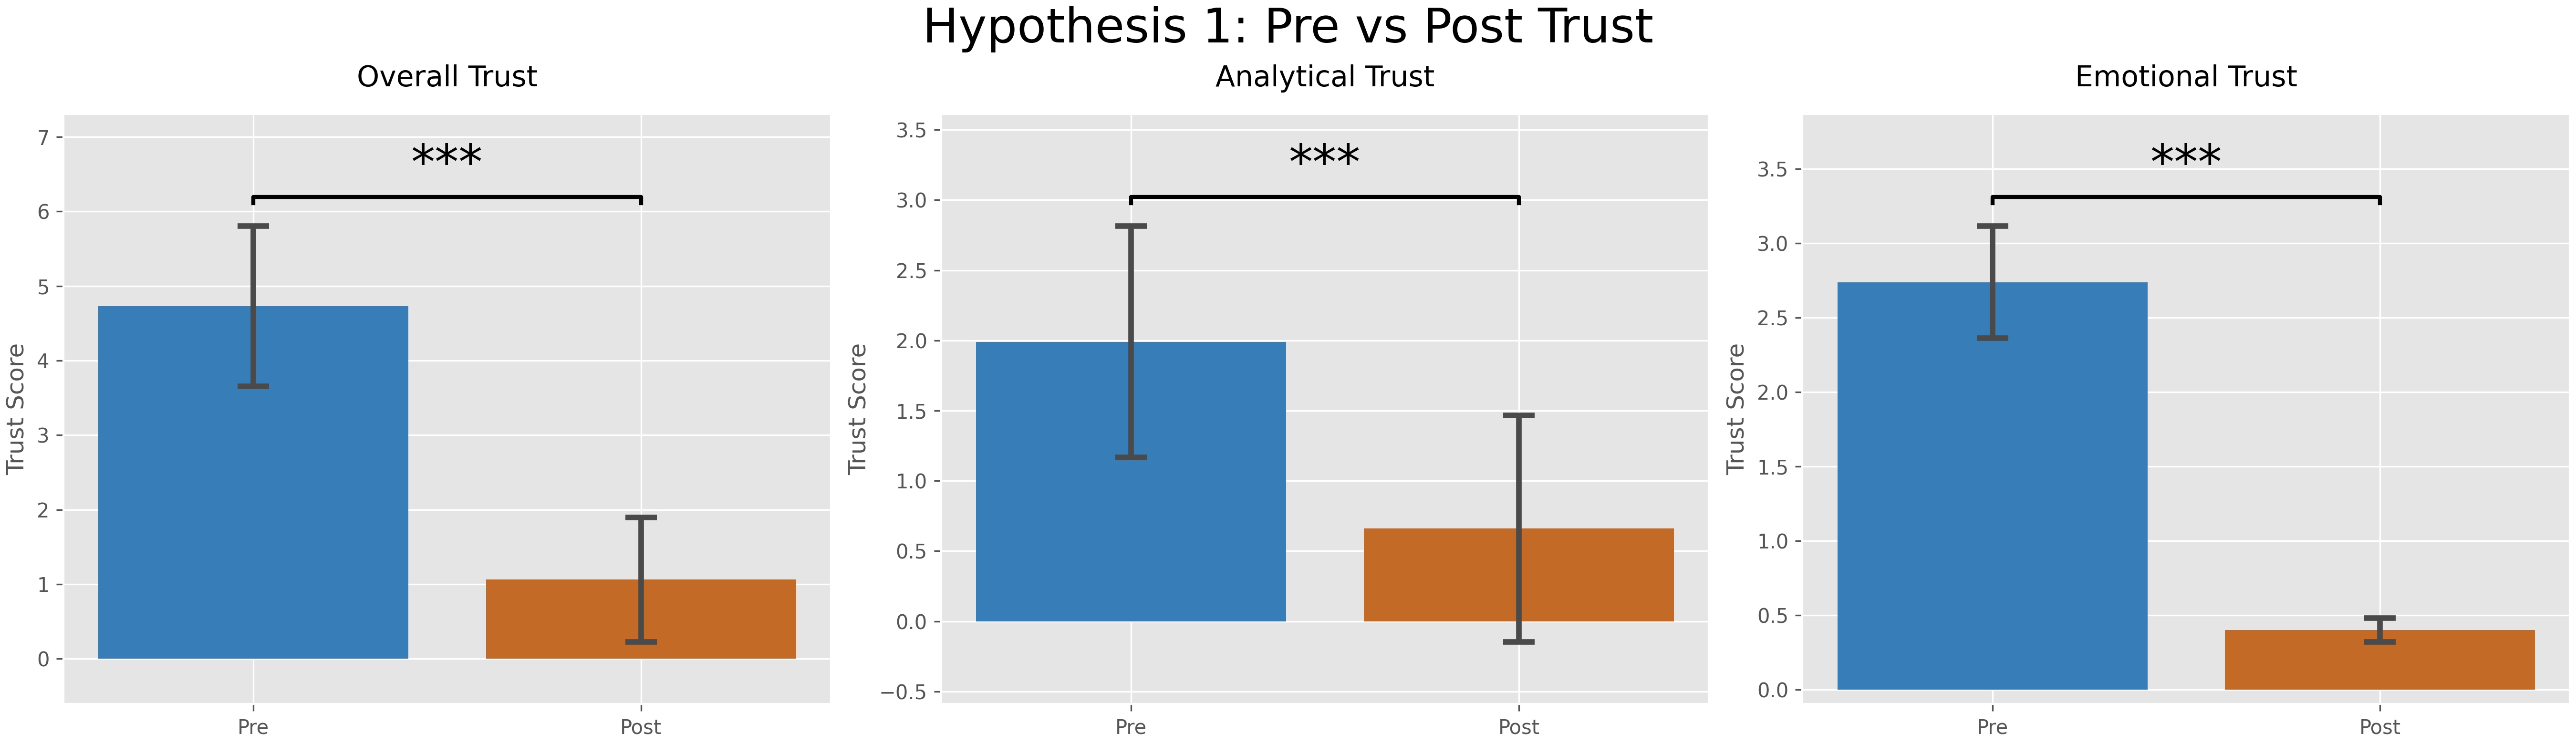
\includegraphics[width=0.85\linewidth]{hypotheses/hypothesis1/hypothesis1.png}
\caption{Visualization for Hypothesis 1.}
\label{fig:hypothesis1}
\end{figure}

\subsubsection{Hypothesis 2}
Hypothesis 2 tested WEIRD participants with four subtests: 2.1 overall pre-post significance, 2.2 analytical pre-post significance, 2.3 emotional pre-post significance, and 2.4 whether emotional and analytical standardized change differ.

2.1 WEIRD Overall pre-post: $n=120$, $M_{pre}=1.217$, $M_{post}=-1.133$, $t(119)=3.440$, $p < .001$, $W=1848.000$, $p_{W} < .001$, $d=-0.314$, $\Delta=-2.350$.
2.2 WEIRD Analytical pre-post: $n=120$, $M_{pre}=-0.167$, $M_{post}=-1.683$, $t(119)=3.014$, $p = .003$, $W=1624.500$, $p_{W} = .003$, $d=-0.275$, $\Delta=-1.517$.
2.3 WEIRD Emotional pre-post: $n=120$, $M_{pre}=1.383$, $M_{post}=0.550$, $t(119)=2.058$, $p = .042$, $W=1936.000$, $p_{W} = .041$, $d=-0.188$, $\Delta=-0.833$.
2.4 WEIRD emotional-vs-analytical standardized change: $n=120$, $M_{em,z}=0.367$, $M_{an,z}=-0.030$, $t(119)=3.301$, $p = .001$, $W=2436.000$, $p_{W} = .002$, $d=0.301$, $\Delta_{z}=0.398$. This supports the predicted significant difference test.

\begin{figure}[h]
\centering
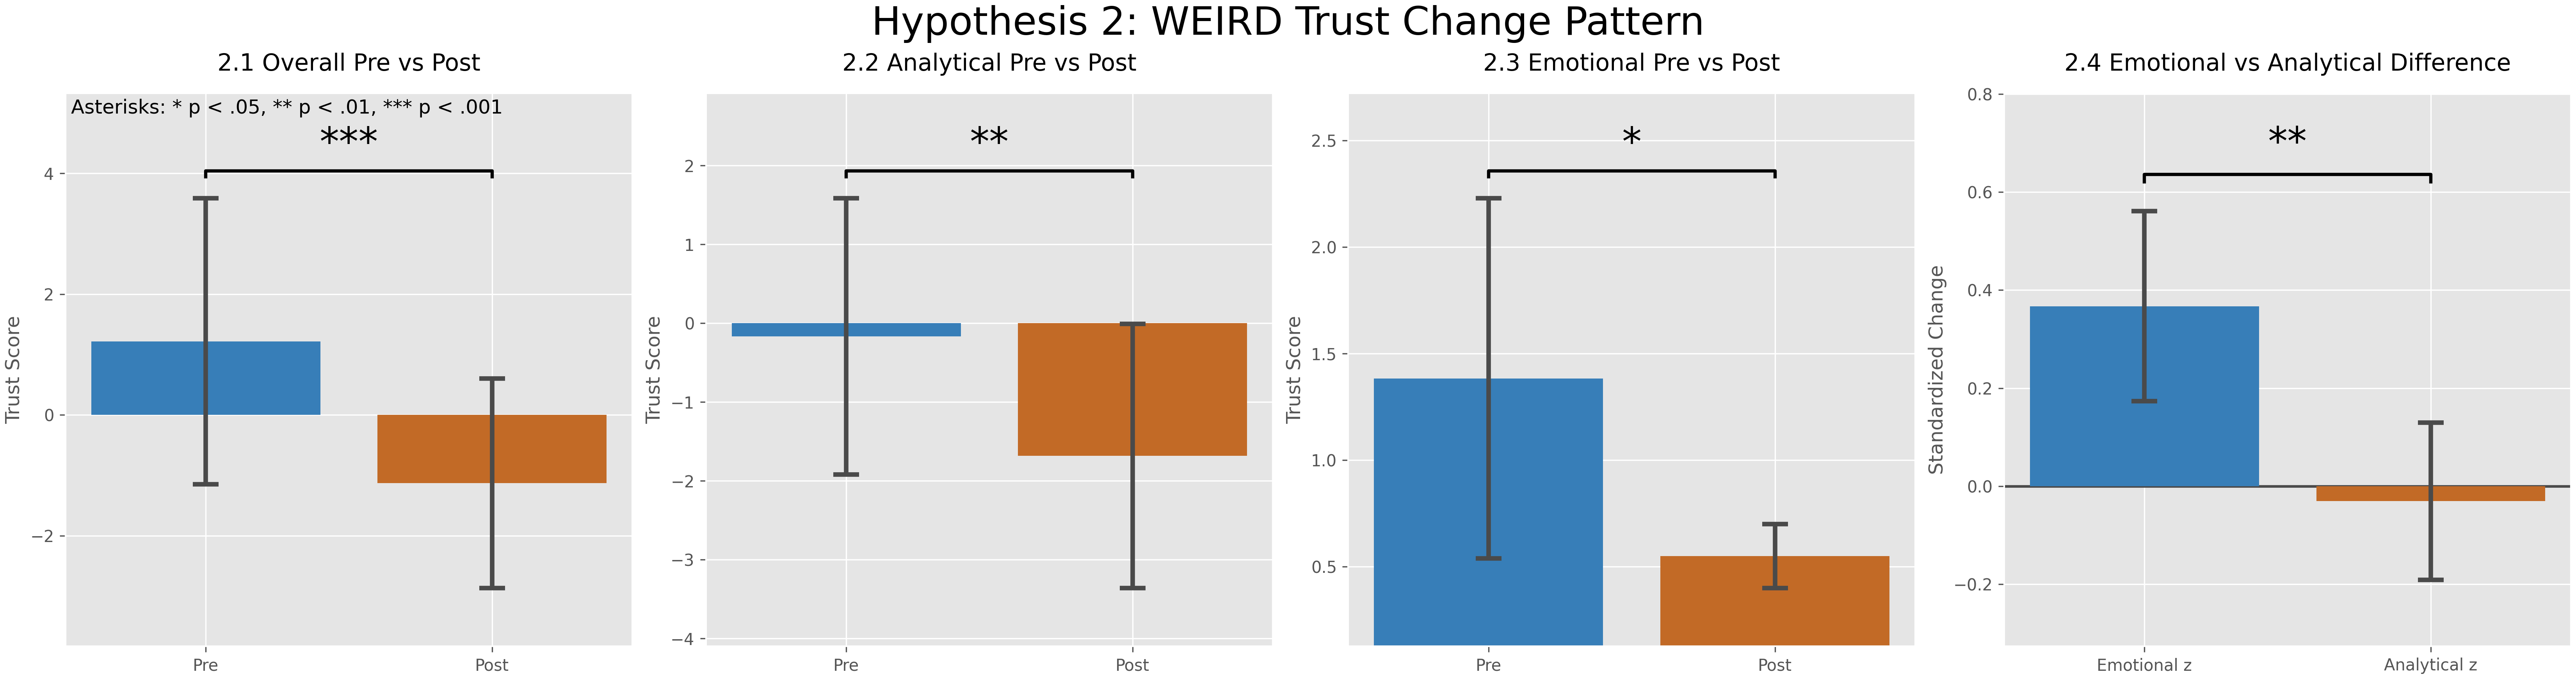
\includegraphics[width=0.85\linewidth]{hypotheses/hypothesis2/hypothesis2.png}
\caption{Visualization for Hypothesis 2.}
\label{fig:hypothesis2}
\end{figure}

\subsubsection{Hypothesis 3}
Hypothesis 3 tested NORMAL/non-WEIRD participants with four subtests: 3.1 overall pre-post significance, 3.2 analytical pre-post significance, 3.3 emotional pre-post significance, and 3.4 whether emotional and analytical standardized change do not differ.

3.1 NORMAL Overall pre-post: $n=384$, $M_{pre}=5.826$, $M_{post}=1.747$, $t(383)=9.970$, $p < .001$, $W=15536.500$, $p_{W} < .001$, $d=-0.509$, $\Delta=-4.078$.
3.2 NORMAL Analytical pre-post: $n=384$, $M_{pre}=2.664$, $M_{post}=1.393$, $t(383)=3.928$, $p < .001$, $W=21912.000$, $p_{W} = .002$, $d=-0.200$, $\Delta=-1.271$.
3.3 NORMAL Emotional pre-post: $n=384$, $M_{pre}=3.161$, $M_{post}=0.354$, $t(383)=14.183$, $p < .001$, $W=6354.500$, $p_{W} < .001$, $d=-0.724$, $\Delta=-2.807$.
3.4 NORMAL emotional-vs-analytical standardized change: $n=384$, $M_{em,z}=-0.115$, $M_{an,z}=0.010$, $t(383)=-1.923$, $p = .055$, $W=32037.000$, $p_{W} = .024$, $d=-0.098$, $\Delta_{z}=-0.124$. This supports the predicted no-difference test.

\begin{figure}[h]
\centering
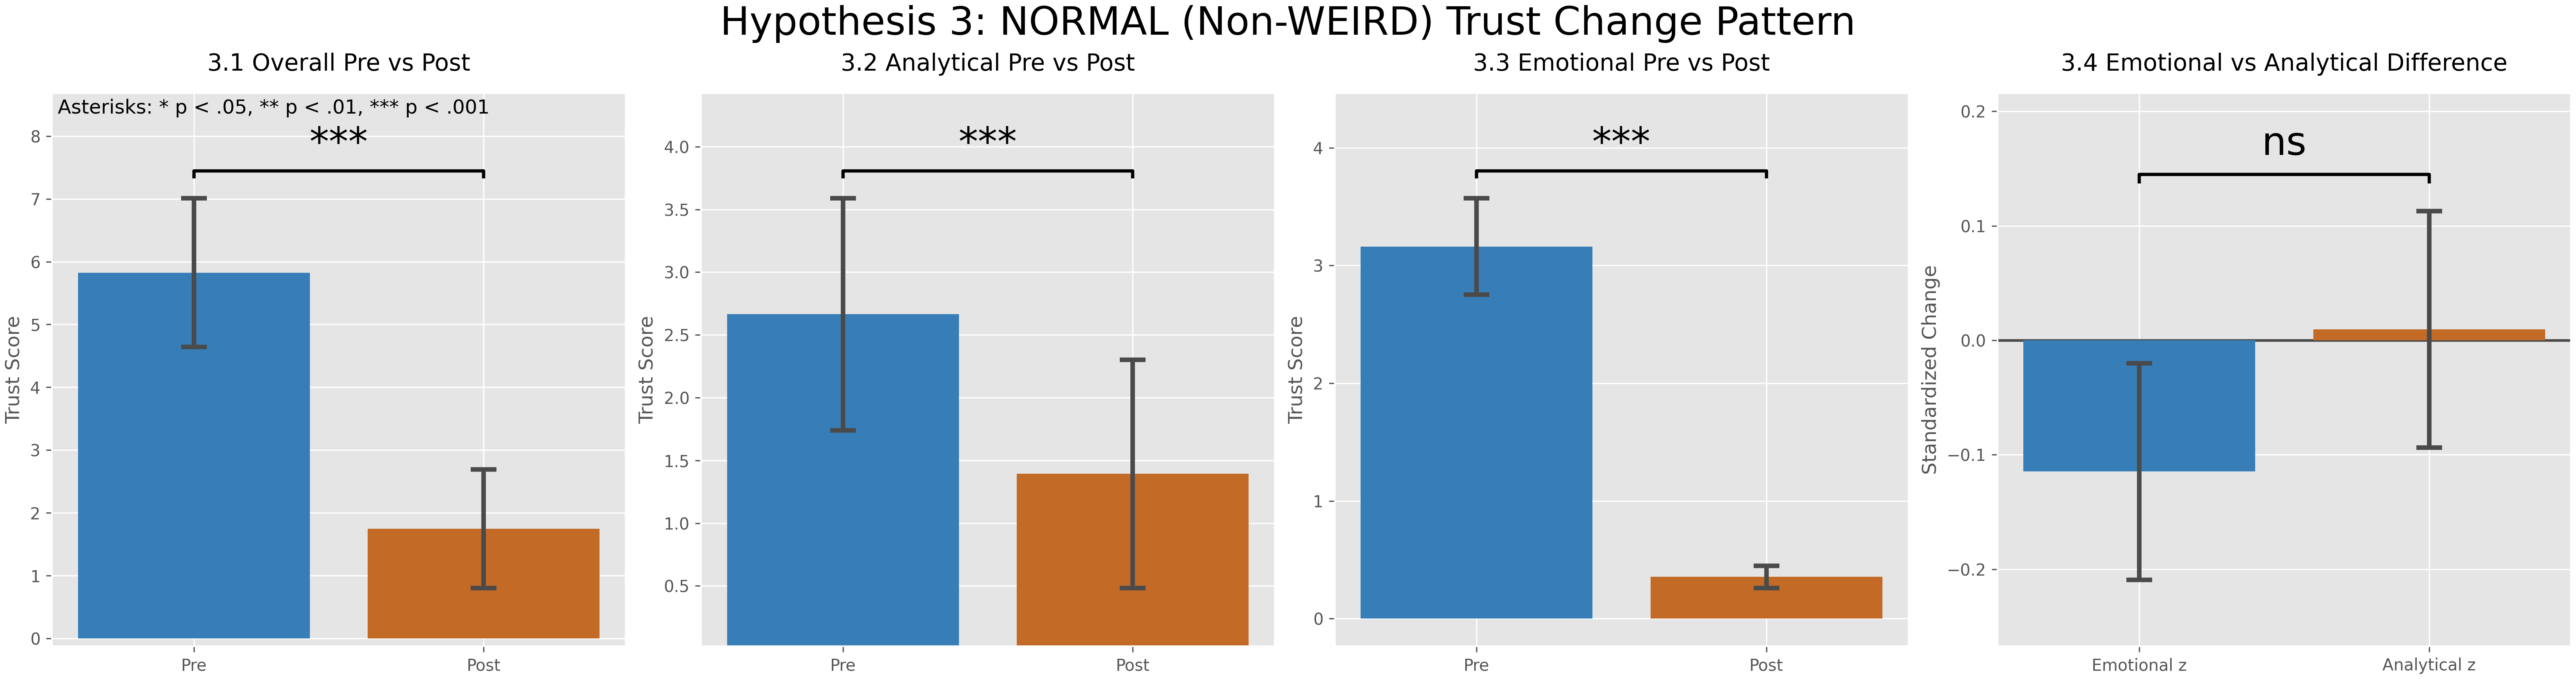
\includegraphics[width=0.85\linewidth]{hypotheses/hypothesis3/hypothesis3.png}
\caption{Visualization for Hypothesis 3.}
\label{fig:hypothesis3}
\end{figure}

\subsubsection{Hypothesis 4}
Hypothesis 4 tested group x condition effects across three trust-change dimensions in a three-panel visualization.
All trust-change outcomes are computed as per-item average change (Post - Pre).

4.1 Analytical trust change by Group x Condition (left panel): paired pre-post tests were WEIRD / Interactive: $t(59)=2.17$, $p = .034$, $\Delta M=-0.180$; WEIRD / Static (Text): $t(59)=2.14$, $p = .037$, $\Delta M=-0.123$; NORMAL / Interactive: $t(191)=2.81$, $p = .006$, $\Delta M=-0.130$; NORMAL / Static (Text): $t(191)=2.74$, $p = .007$, $\Delta M=-0.124$. Omnibus four-cell ANOVA: $F=0.14$, $p = .938$. Interaction estimate: $b=-0.050$, $t(500)=-0.39$, $p = .696$.
4.2 Emotional trust change by Group x Condition (middle panel): paired pre-post tests were WEIRD / Interactive: $t(59)=1.71$, $p = .092$, $\Delta M=-0.104$; WEIRD / Static (Text): $t(59)=1.22$, $p = .229$, $\Delta M=-0.081$; NORMAL / Interactive: $t(191)=9.48$, $p < .001$, $\Delta M=-0.297$; NORMAL / Static (Text): $t(191)=10.57$, $p < .001$, $\Delta M=-0.326$. Omnibus four-cell ANOVA: $F=7.49$, $p < .001$. Interaction estimate: $b=-0.051$, $t(500)=-0.55$, $p = .585$.
4.3 Analytical-vs-emotional change difference by Group x Condition (right panel): Welch tests by condition were Interactive: $t=-2.28$, $p = .025$, $M_{WEIRD}=-0.076$, $M_{NORMAL}=0.167$; Static (Text): $t=-2.46$, $p = .015$, $M_{WEIRD}=-0.042$, $M_{NORMAL}=0.202$. Omnibus four-cell ANOVA: $F=3.82$, $p = .010$. Interaction estimate: $b=0.001$, $t(500)=0.01$, $p = .996$.
Asterisk key: * p < .05, ** p < .01, *** p < .001.

\begin{figure}[h]
\centering
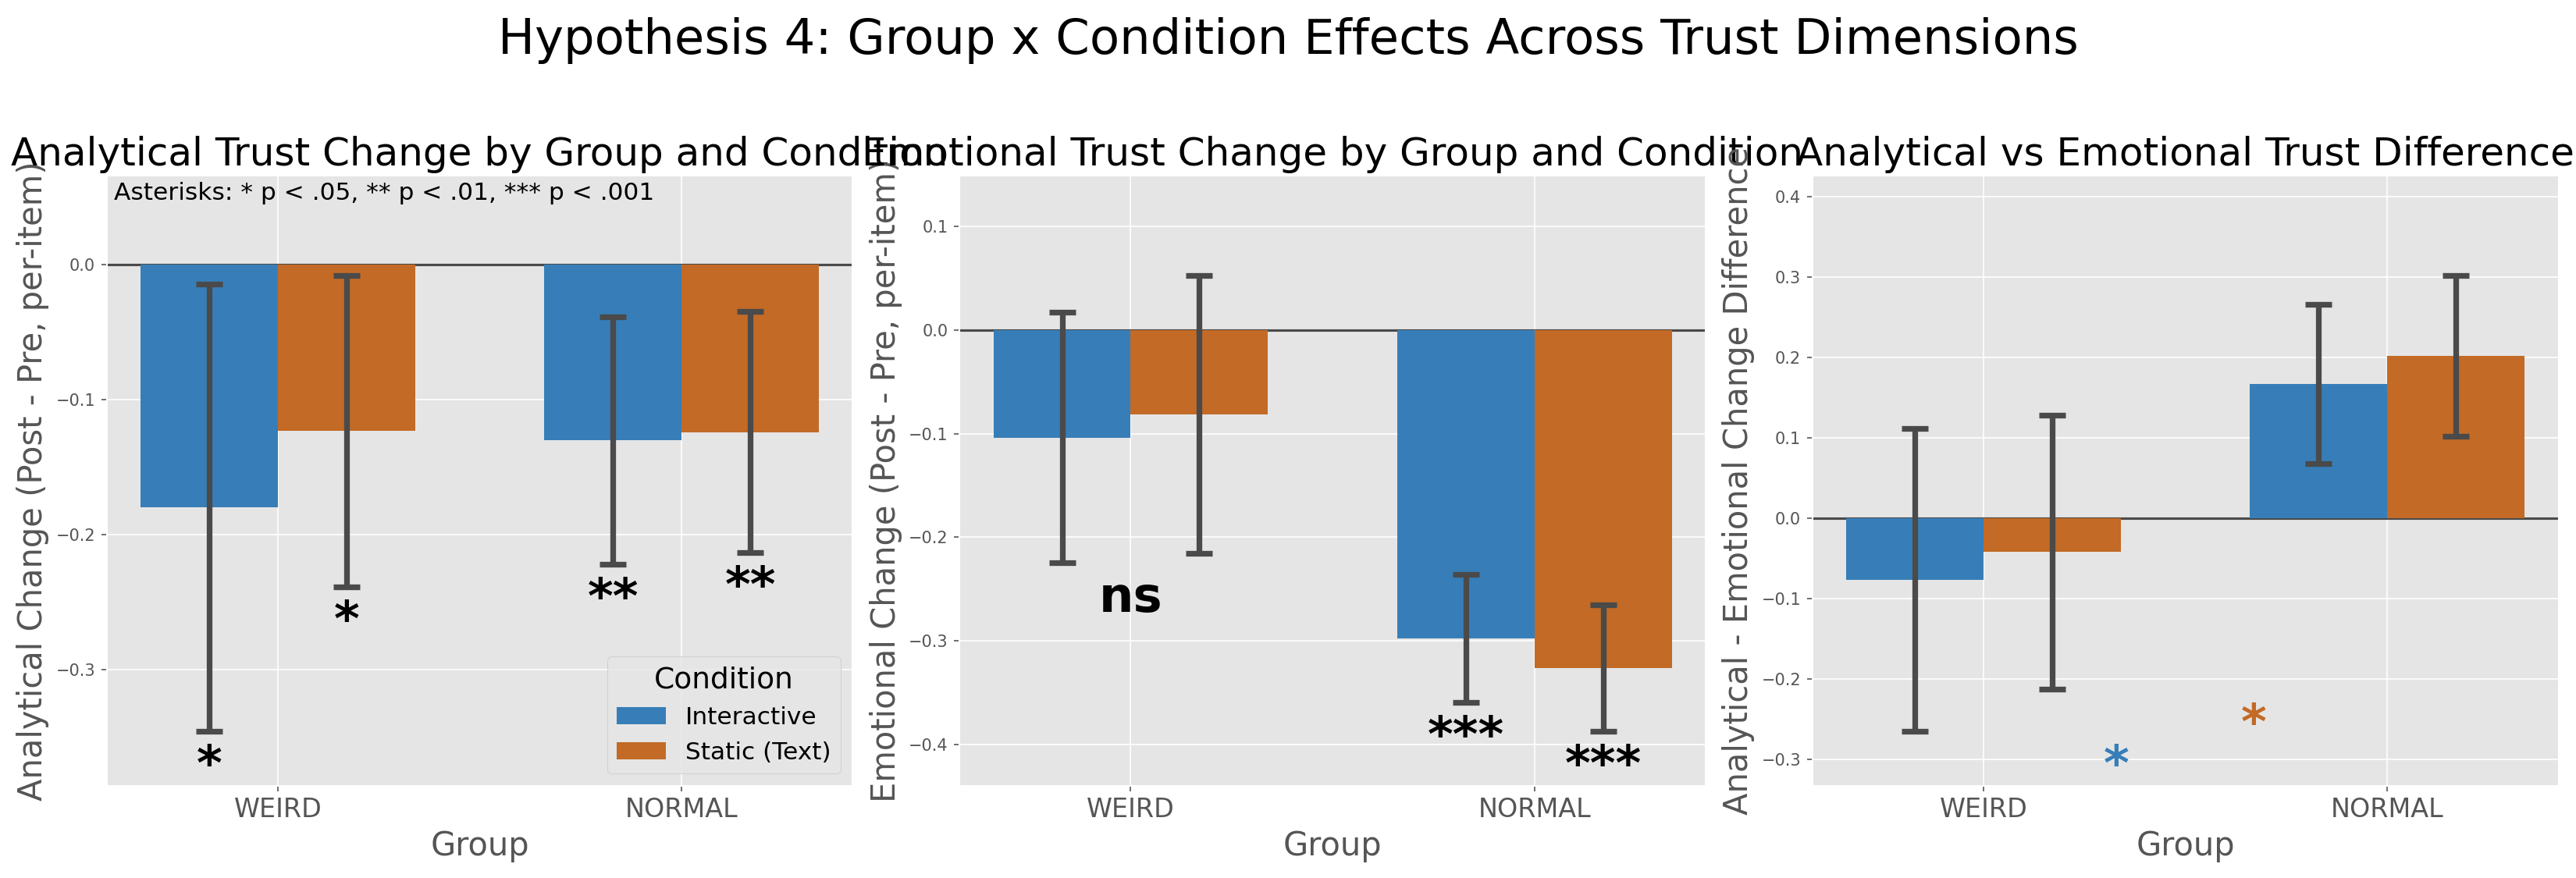
\includegraphics[width=0.85\linewidth]{hypotheses/hypothesis4/hypothesis4.png}
\caption{Visualization for Hypothesis 4.}
\label{fig:hypothesis4}
\end{figure}

\subsubsection{Hypothesis 5}
Hypothesis 5 compared WEIRD and NORMAL participants on standardized change metrics: emotional standardized change, analytical standardized change, and overall standardized change.

5.1 WEIRD vs NORMAL emotional standardized change: $n_{WEIRD}=120$, $n_{NORMAL}=384$, $M_{WEIRD}=0.367$, $M_{NORMAL}=-0.115$, $t=4.380$, $p < .001$, $\Delta(M_W-M_N)=0.482$.
5.2 WEIRD vs NORMAL analytical standardized change: $n_{WEIRD}=120$, $n_{NORMAL}=384$, $M_{WEIRD}=-0.030$, $M_{NORMAL}=0.010$, $t=-0.411$, $p = .682$, $\Delta(M_W-M_N)=-0.040$.
5.3 WEIRD vs NORMAL overall standardized change: $n_{WEIRD}=120$, $n_{NORMAL}=384$, $M_{WEIRD}=0.166$, $M_{NORMAL}=-0.052$, $t=2.170$, $p = .031$, $\Delta(M_W-M_N)=0.218$.
Asterisk key: * p < .05, ** p < .01, *** p < .001.

\begin{figure}[h]
\centering

\includegraphics[width=0.85\linewidth]{hypotheses/hypothesis5/hypothesis5.png}
\caption{Visualization for Hypothesis 5.}
\label{fig:hypothesis5}
\end{figure}

\subsubsection{Hypothesis 6}
Hypothesis 6 tested whether Interactive and Static (Text) explanations produced different analytical and emotional trust-change outcomes, including demographic coverage, WEIRD/NORMAL subgroup tests, and analytical-vs-emotional comparisons.

6.1 Across both trust types and demographics:
Overall condition effect (analytical): $M_{Interactive}=-0.142$, $M_{Text}=-0.124$, $t=-0.333$, $p = .739$.
Overall condition effect (emotional): $M_{Interactive}=-0.251$, $M_{Text}=-0.268$, $t=0.412$, $p = .680$.
Demographic-adjusted OLS condition effect (analytical): $b=-0.034$, $SE=0.054$, $t(473)=-0.636$, $p = .525$, $R^2=0.128$.
Demographic-adjusted OLS condition effect (emotional): $b=0.014$, $SE=0.038$, $t(473)=0.359$, $p = .720$, $R^2=0.200$.
Significant demographic-stratified Interactive vs Text effects (p < .05):
- Analytical change:
  Nationality Top=Canada: $\Delta(M_I-M_T)=-0.512$, $t=-2.513$, $p = .019$.
  Gender Norm=Woman: $\Delta(M_I-M_T)=-0.171$, $t=-1.996$, $p = .048$.
- Emotional change:
  Ethnicity Norm=Asian: $\Delta(M_I-M_T)=0.195$, $t=2.113$, $p = .037$.

6.2 Between WEIRD and NORMAL:
Analytical condition effect within WEIRD: $M_I=-0.180$, $M_T=-0.123$, $t=-0.561$, $p = .576$.
Analytical condition effect within NORMAL: $M_I=-0.130$, $M_T=-0.124$, $t=-0.096$, $p = .923$.
Emotional condition effect within WEIRD: $M_I=-0.104$, $M_T=-0.081$, $t=-0.246$, $p = .806$.
Emotional condition effect within NORMAL: $M_I=-0.297$, $M_T=-0.326$, $t=0.657$, $p = .511$.
Analytical group x condition interaction: $b=-0.050$, $t(500)=-0.391$, $p = .696$.
Emotional group x condition interaction: $b=-0.051$, $t(500)=-0.547$, $p = .585$.

6.3 Between analytical vs emotional trust:
Interactive paired analytical vs emotional: $M_A=-0.142$, $M_E=-0.251$, $t(251)=2.439$, $p = .015$.
Static (Text) paired analytical vs emotional: $M_A=-0.124$, $M_E=-0.268$, $t(251)=3.281$, $p = .001$.
Condition contrast on analytical-emotional difference score: $M_I=0.109$, $M_T=0.144$, $t=-0.558$, $p = .577$.
Asterisk key: * p < .05, ** p < .01, *** p < .001.

\begin{figure}[h]
\centering

\includegraphics[width=0.85\linewidth]{hypotheses/hypothesis6/hypothesis6.png}
\caption{Visualization for Hypothesis 6.}
\label{fig:hypothesis6}
\end{figure}

\subsubsection{Hypothesis 7}
Hypothesis 7 tested whether there is a main effect of condition across three trust-change outcomes: overall change, emotional change, and analytical change.

7.1 Main condition effect on overall change:
Overall change condition effect: $M_{Interactive}=-0.197$, $M_{Text}=-0.196$, $t=-0.020$, $p = .984$, $\Delta(M_I-M_T)=-0.001$.
Interpretation: no significant main condition effect on overall change.

7.2 Main condition effect on emotional change:
Emotional change condition effect: $M_{Interactive}=-0.251$, $M_{Text}=-0.268$, $t=0.412$, $p = .680$, $\Delta(M_I-M_T)=0.017$.
Interpretation: no significant main condition effect on emotional change.

7.3 Main condition effect on analytical change:
Analytical change condition effect: $M_{Interactive}=-0.142$, $M_{Text}=-0.124$, $t=-0.333$, $p = .739$, $\Delta(M_I-M_T)=-0.018$.
Interpretation: no significant main condition effect on analytical change.
Asterisk key: * p < .05, ** p < .01, *** p < .001.

\begin{figure}[h]
\centering
\includegraphics[width=0.85\linewidth]{hypotheses/hypothesis7/hypothesis7.png}
\caption{Visualization for Hypothesis 7.}
\label{fig:hypothesis7}
\end{figure}

\subsubsection{Hypothesis 8}
Hypothesis 8 tested whether the main effect of condition differs across overall, emotional, and analytical trust change when analyzed separately within WEIRD and NORMAL participants.

8.1 Main condition effect on overall change (split by WEIRD/NORMAL):
- WEIRD: $n_{Interactive}=60$, $n_{Text}=60$, $M_{Interactive}=-0.142$, $M_{Text}=-0.102$, $t=-0.550$, $p = .583$, $\Delta(M_I-M_T)=-0.039$.
- NORMAL: $n_{Interactive}=192$, $n_{Text}=192$, $M_{Interactive}=-0.214$, $M_{Text}=-0.225$, $t=0.268$, $p = .789$, $\Delta(M_I-M_T)=0.011$.
Interpretation: no significant condition effect detected in either WEIRD or NORMAL.

8.2 Main condition effect on emotional change (split by WEIRD/NORMAL):
- WEIRD: $n_{Interactive}=60$, $n_{Text}=60$, $M_{Interactive}=-0.104$, $M_{Text}=-0.081$, $t=-0.246$, $p = .806$, $\Delta(M_I-M_T)=-0.022$.
- NORMAL: $n_{Interactive}=192$, $n_{Text}=192$, $M_{Interactive}=-0.297$, $M_{Text}=-0.326$, $t=0.657$, $p = .511$, $\Delta(M_I-M_T)=0.029$.
Interpretation: no significant condition effect detected in either WEIRD or NORMAL.

8.3 Main condition effect on analytical change (split by WEIRD/NORMAL):
- WEIRD: $n_{Interactive}=60$, $n_{Text}=60$, $M_{Interactive}=-0.180$, $M_{Text}=-0.123$, $t=-0.561$, $p = .576$, $\Delta(M_I-M_T)=-0.057$.
- NORMAL: $n_{Interactive}=192$, $n_{Text}=192$, $M_{Interactive}=-0.130$, $M_{Text}=-0.124$, $t=-0.096$, $p = .923$, $\Delta(M_I-M_T)=-0.006$.
Interpretation: no significant condition effect detected in either WEIRD or NORMAL.
Asterisk key: * p < .05, ** p < .01, *** p < .001.

\begin{figure}[h]
\centering
\includegraphics[width=0.85\linewidth]{hypotheses/hypothesis8/hypothesis8.png}
\caption{Visualization for Hypothesis 8.}
\label{fig:hypothesis8}
\end{figure}

\subsubsection{Hypothesis 9}
Hypothesis 9 tested whether the condition effect on trust-change magnitude depends on the interaction between WEIRD vs NORMAL grouping and trust type (analytical vs emotional), operationalized as analytical-minus-emotional change.

9.1 Condition effect on analytical-minus-emotional change within WEIRD participants:
- WEIRD: $n_{Interactive}=60$, $n_{Text}=60$, $M_{Interactive}=-0.076$, $M_{Text}=-0.042$, $t=-0.271$, $p = .787$, $\Delta(M_I-M_T)=-0.034$.
Interpretation: no significant condition effect within WEIRD participants.

9.2 Condition effect on analytical-minus-emotional change within NORMAL participants:
- NORMAL: $n_{Interactive}=192$, $n_{Text}=192$, $M_{Interactive}=0.167$, $M_{Text}=0.202$, $t=-0.493$, $p = .622$, $\Delta(M_I-M_T)=-0.035$.
Interpretation: no significant condition effect within NORMAL participants.

9.3 Group x Condition interaction on analytical-minus-emotional change:
Interaction estimate: $b=0.001$, $t(500)=0.005$, $p = .996$.
Interpretation: no significant evidence that the condition effect differs between WEIRD and NORMAL participants.

9.4 Long-form Condition x Group x Trust-Type model on trust change:
Three-way interaction estimate (Condition x Group x Trust Type): $b=-0.001$, $t(1000)=-0.005$, $p = .996$, $n_{obs}=1008$, $n_{participants}=504$.
Interpretation: no significant three-way interaction in the long-form model.
Asterisk key: * p < .05, ** p < .01, *** p < .001.

\begin{figure}[h]
\centering

\includegraphics[width=0.85\linewidth]{hypotheses/hypothesis9/hypothesis9.png}
\caption{Visualization for Hypothesis 9.}
\label{fig:hypothesis9}
\end{figure}

\subsubsection{Hypothesis 10}
Hypothesis 10 tested whether WEIRD and NORMAL participants differ in pre-experiment overall trust, analytical trust, and emotional trust.

10.1 WEIRD vs NORMAL difference in pre-experiment overall trust:
Overall pre-trust group contrast: $n_{WEIRD}=120$, $n_{NORMAL}=384$, $M_{WEIRD}=1.217$, $M_{NORMAL}=5.826$, $t=-3.412$, $p < .001$, $\Delta(M_W-M_N)=-4.609$.
Interpretation: significant WEIRD vs NORMAL difference in pre-experiment overall trust.

10.2 WEIRD vs NORMAL difference in pre-experiment analytical trust:
Analytical pre-trust group contrast: $n_{WEIRD}=120$, $n_{NORMAL}=384$, $M_{WEIRD}=-0.167$, $M_{NORMAL}=2.664$, $t=-2.802$, $p = .006$, $\Delta(M_W-M_N)=-2.831$.
Interpretation: significant WEIRD vs NORMAL difference in pre-experiment analytical trust.

10.3 WEIRD vs NORMAL difference in pre-experiment emotional trust:
Emotional pre-trust group contrast: $n_{WEIRD}=120$, $n_{NORMAL}=384$, $M_{WEIRD}=1.383$, $M_{NORMAL}=3.161$, $t=-3.715$, $p < .001$, $\Delta(M_W-M_N)=-1.778$.
Interpretation: significant WEIRD vs NORMAL difference in pre-experiment emotional trust.
Asterisk key: * p < .05, ** p < .01, *** p < .001.

\begin{figure}[h]
\centering

\includegraphics[width=0.85\linewidth]{hypotheses/hypothesis10/hypothesis10.png}
\caption{Visualization for Hypothesis 10.}
\label{fig:hypothesis10}
\end{figure}

\subsubsection{Hypothesis 11}
Hypothesis 11 tested whether WEIRD and NORMAL participants differ in post-experiment overall trust, analytical trust, and emotional trust.

11.1 WEIRD vs NORMAL difference in post-experiment overall trust:
Overall post-trust group contrast: $n_{WEIRD}=120$, $n_{NORMAL}=384$, $M_{WEIRD}=-1.133$, $M_{NORMAL}=1.747$, $t=-2.862$, $p = .005$, $\Delta(M_W-M_N)=-2.881$.
Interpretation: significant WEIRD vs NORMAL difference in post-experiment overall trust.

11.2 WEIRD vs NORMAL difference in post-experiment analytical trust:
Analytical post-trust group contrast: $n_{WEIRD}=120$, $n_{NORMAL}=384$, $M_{WEIRD}=-1.683$, $M_{NORMAL}=1.393$, $t=-3.165$, $p = .002$, $\Delta(M_W-M_N)=-3.077$.
Interpretation: significant WEIRD vs NORMAL difference in post-experiment analytical trust.

11.3 WEIRD vs NORMAL difference in post-experiment emotional trust:
Emotional post-trust group contrast: $n_{WEIRD}=120$, $n_{NORMAL}=384$, $M_{WEIRD}=0.550$, $M_{NORMAL}=0.354$, $t=2.170$, $p = .031$, $\Delta(M_W-M_N)=0.196$.
Interpretation: significant WEIRD vs NORMAL difference in post-experiment emotional trust.
Asterisk key: * p < .05, ** p < .01, *** p < .001.

\begin{figure}[h]
\centering

\includegraphics[width=0.85\linewidth]{hypotheses/hypothesis11/hypothesis11.png}
\caption{Visualization for Hypothesis 11.}
\label{fig:hypothesis11}
\end{figure}

\subsubsection{Hypothesis 12}
Hypothesis 12 tested whether WEIRD and NORMAL participants differ in pre-to-post trust change using Group x Time interaction models (difference-in-differences) for overall, analytical, and emotional trust.

12.1 Group x Time interaction for overall trust:
WEIRD pre-post: $n=120$, $\Delta(M_{post}-M_{pre})=-2.350$, $t=3.440$, $p < .001$.
NORMAL pre-post: $n=384$, $\Delta(M_{post}-M_{pre})=-4.078$, $t=9.970$, $p < .001$.
Interaction estimate: $b=1.728$, $t(1004)=1.070$, $p = .285$.

12.2 Group x Time interaction for analytical trust:
WEIRD pre-post: $n=120$, $\Delta(M_{post}-M_{pre})=-1.517$, $t=3.014$, $p = .003$.
NORMAL pre-post: $n=384$, $\Delta(M_{post}-M_{pre})=-1.271$, $t=3.928$, $p < .001$.
Interaction estimate: $b=-0.246$, $t(1004)=-0.179$, $p = .858$.

12.3 Group x Time interaction for emotional trust:
WEIRD pre-post: $n=120$, $\Delta(M_{post}-M_{pre})=-0.833$, $t=2.058$, $p = .042$.
NORMAL pre-post: $n=384$, $\Delta(M_{post}-M_{pre})=-2.807$, $t=14.183$, $p < .001$.
Interaction estimate: $b=1.974$, $t(1004)=4.345$, $p < .001$.
Asterisk key: * p < .05, ** p < .01, *** p < .001.

\begin{figure}[h]
\centering

\includegraphics[width=0.85\linewidth]{hypotheses/hypothesis12/hypothesis12.png}
\caption{Visualization for Hypothesis 12.}
\label{fig:hypothesis12}
\end{figure}

